\documentclass[11pt,a4paper]{article}

\usepackage[margin=1in]{geometry}
\usepackage{amsmath,amssymb,amsthm}
\usepackage{booktabs}
\usepackage{enumitem}
\usepackage{graphicx}
\usepackage{hyperref}
\usepackage{parskip}

\hypersetup{colorlinks=true, linkcolor=blue, urlcolor=blue}

\newtheorem{theorem}{Theorem}
\newtheorem{claim}{Claim}
\newtheorem{remark}[theorem]{Remark}

\newcommand{\keyidea}[1]{\medskip\noindent\textbf{Key idea.}\ #1\medskip}
\newcommand{\econ}[1]{\medskip\noindent\textbf{Economics.}\ #1\medskip}

\title{\textbf{Duality Theory Notes}\\[0.2em]
\large Math Camp 2026 --- Teaching Notes}
\author{}
\date{}

\begin{document}
\maketitle

\begin{center}
\small
\textit{Primal: pick inputs to minimize cost while meeting output targets.\\
Dual: find the best lower bound on that minimum using shadow prices on outputs.}
\end{center}

\tableofcontents
\newpage

%==============================================================================
\section{Why duality?}
%==============================================================================

Many economic problems are \textbf{cost-minimization} problems: a firm chooses how much labor, material,
and other inputs to use, pays for them, and must produce at least given amounts of each output.
Before computing an optimum, ask a simpler question: how low could cost \emph{possibly} be, given only
the technology and the output targets?

\keyidea{Before solving exactly, ask: \emph{what is the best lower bound we can prove on minimum cost?}
Duality turns that bound into a \textbf{second optimization problem} whose variables are
\textbf{shadow prices} on the outputs.}

\textbf{The cast of characters.}
\begin{itemize}[nosep,leftmargin=*]
  \item \textbf{Inputs} (labor hours, tons of material, machine time): what the firm uses and pays for.
  \item \textbf{Input costs}: the dollar price per unit of each input.
  \item \textbf{Output targets}: minimum amounts of each good that must be produced.
  \item \textbf{Technology}: how much of each output one unit of each input creates.
  \item \textbf{Shadow prices on outputs}: internal dollar values assigned to each good in a valuation
        exercise (not necessarily market prices).
\end{itemize}

\textbf{Worked example (two inputs, two outputs).}
Labor costs \$3 per hour; material costs \$5 per ton.
Targets: at least 4 widgets and 6 gadgets.
Technology (rows: widgets, gadgets; columns: labor per hour, material per ton):
\[
  \begin{pmatrix}
    1 & 0 \\[4pt]
    \tfrac12 & 2
  \end{pmatrix}
\]
Input costs, output targets, and one feasible input mix:
\[
  \text{costs}=
  \begin{pmatrix} 3 \\ 5 \end{pmatrix},
  \qquad
  \text{targets}=
  \begin{pmatrix} 4 \\ 6 \end{pmatrix},
  \qquad
  \text{plan}=
  \begin{pmatrix} 4 \\ 2 \end{pmatrix}
  \quad
  \text{(4 labor-hours, 2 tons of material).}
\]
Total cost: $4\times 3 + 2\times 5 = 22$.
Widgets produced: $4\times 1 + 2\times 0 = 4$.
Gadgets produced: $4\times\tfrac12 + 2\times 2 = 6$.
The \textbf{planner} asks: what is the cheapest feasible input mix?
The \textbf{accountant} asks: what is the highest total value we can assign to the output targets without
making any input look like a bargain at those internal output prices?

\textbf{Connecting output value to a cost floor (intuition only).}
The accountant assigns a dollar value to each output type (widget price, gadget price) and defines
\[
  V = \text{(widget price)}\times 4 + \text{(gadget price)}\times 6,
\]
the paper value of the \emph{targets} (4 widgets and 6 gadgets).
The claim we want is: \textbf{every feasible plan has real input cost at least~$V$.}

To get there, compare three numbers for \textbf{any} feasible production plan:

\begin{center}
\small
\begin{tabular}{cl}
\textbf{Real input bill} & what you actually pay for labor and material \\[2pt]
$\downarrow$ \textbf{Link 1} & \\[2pt]
\textbf{Accounting value produced} & widget price $\times$ widgets made + gadget price $\times$ gadgets made \\[2pt]
$\downarrow$ \textbf{Link 2} & \\[2pt]
\textbf{Value of targets} ($V$) & widget price $\times$ 4 + gadget price $\times$ 6 \\
\end{tabular}
\end{center}

\emph{Link 1: real input bill $\ge$ accounting value of what was produced.}
You pay for inputs; those inputs create outputs; each output has an accounting price.
\textbf{Link 1} says the total bill cannot be \emph{below} the accounting value of what came out.
It holds only if output prices are \textbf{consistent}: check each input separately.
One hour of labor costs \$3; at your internal prices it creates
$1\times(\text{widget price}) + \tfrac12\times(\text{gadget price})$ of value.
If that exceeded \$3, labor would be a money machine---so consistent prices rule that out.
Same check for material (\$5 per ton). Add over all inputs used.

\emph{Link 2: accounting value of what was produced $\ge V$.}
The plan meets the targets (at least 4 widgets and 6 gadgets), and output prices are nonnegative.
So the accounting value of what you \emph{actually} produced is at least the accounting value of the
\emph{minimum required} amounts---that is exactly~$V$.

\emph{Chain.}
Link 1 and Link 2 together give
\[
  \text{real input bill}
  \;\ge\;
  \text{accounting value produced}
  \;\ge\;
  V.
\]
So every feasible plan costs at least~$V$; the true minimum cannot be below~$V$.
\textbf{Duality} asks the accountant to raise $V$ as high as possible while keeping prices consistent.
At the optimum, planner and accountant agree on the number.

\smallskip
\noindent\emph{(If this story does not click yet, that is fine---Section~2 gives the formal math.
You can treat this section as motivation only.)}

The next section makes this precise for linear programs: we introduce notation, derive the primal--dual pair,
prove that dual values are valid lower bounds, and show that the best dual value equals the primal optimum.

%==============================================================================
\section{Linear programming duality}
%==============================================================================

We build LP duality in four steps.
First, derive the dual from a lower-bound argument.
Second, prove \textbf{weak duality} (dual $\le$ primal).
Third, prove \textbf{strong duality} (dual $=$ primal), using Farkas' Lemma as the key tool.
Fourth, read optimality through \textbf{complementary slackness} and extend the recipe to general LPs.

\textbf{The primal--dual pair.}
The \textbf{primal} in input--output form is
\begin{equation}\label{eq:primal}
  \text{(P)}\quad
  \min\ \mathbf{c}^{\mathsf T}\mathbf{x}
  \quad\text{s.t.}\quad A\mathbf{x}\ge\mathbf{b},\ \mathbf{x}\ge\mathbf{0}.
\end{equation}
We now turn the informal lower-bound idea into an explicit dual problem.

\begin{claim}[Dual of the standard LP]
Problem~\eqref{eq:dual} is the best LP lower bound on the optimum of~\eqref{eq:primal} obtained by
nonnegative shadow prices on the constraints:
\begin{equation}\label{eq:dual}
  \text{(D)}\quad
  \max\ \mathbf{b}^{\mathsf T}\mathbf{y}
  \quad\text{s.t.}\quad A^{\mathsf T}\mathbf{y}\le\mathbf{c},\ \mathbf{y}\ge\mathbf{0}.
\end{equation}
\end{claim}

\begin{proof}
Pick any $\mathbf{y}\ge\mathbf{0}$.
From $A\mathbf{x}\ge\mathbf{b}$, multiplying row $i$ by $y_i\ge 0$ and summing gives
$\mathbf{y}^{\mathsf T}A\mathbf{x}\ge\mathbf{b}^{\mathsf T}\mathbf{y}$.
If also $A^{\mathsf T}\mathbf{y}\le\mathbf{c}$, then for every $\mathbf{x}\ge\mathbf{0}$,
\[
  \mathbf{c}^{\mathsf T}\mathbf{x}\ge \mathbf{y}^{\mathsf T}A\mathbf{x}
  \ge \mathbf{b}^{\mathsf T}\mathbf{y}.
\]
So $\mathbf{b}^{\mathsf T}\mathbf{y}$ is a lower bound on primal cost for every feasible $\mathbf{x}$.
Maximising this bound over $\mathbf{y}$ gives~\eqref{eq:dual}.
\end{proof}

\econ{Read the pair as follows.
\begin{itemize}[nosep,leftmargin=*]
  \item $x_j$: quantity of input $j$ (labor, material);\quad $c_j$: its unit cost.
  \item $(A\mathbf{x})_i\ge b_i$: output of type $i$ meets the target.
  \item $y_i$: \textbf{shadow price} of output $i$.
  \item $A^{\mathsf T}\mathbf{y}\le\mathbf{c}$: value of outputs attributable to each input $\le$ its cost.
  \item $\mathbf{b}^{\mathsf T}\mathbf{y}$: total value of output targets at prices $\mathbf{y}$.
\end{itemize}}

A small illustration fixes the notation (one output type, so $A$ is a single row).
Consider $\min\ 3x_1+5x_2$ s.t.\ $x_1+2x_2\ge 4$, $x_1,x_2\ge 0$, i.e.\ $A=(1\ \ 2)$:
one unit of labor yields $a_{11}=1$ unit of output, one unit of material yields $a_{12}=2$ units.
($x_1$ = labor, $x_2$ = material; produce at least 4 units at minimum cost).
The dual is $\max\ 4y$ s.t.\ $y\le 3$, $2y\le 5$, $y\ge 0$, which gives $y^*=3$ and cost $=12$.

Having defined the pair, the first theorem says that every feasible dual solution gives a valid bound.

\textbf{Weak duality.}

\begin{theorem}[Weak duality]
For every feasible $\mathbf{x}$ of~\eqref{eq:primal} and $\mathbf{y}$ of~\eqref{eq:dual},
$\mathbf{c}^{\mathsf T}\mathbf{x}\ge\mathbf{b}^{\mathsf T}\mathbf{y}$, hence $p^*\ge d^*$.
\end{theorem}

\begin{proof}
Dual feasibility gives $A^{\mathsf T}\mathbf{y}\le\mathbf{c}$.
Since $\mathbf{x}\ge\mathbf{0}$, we get $\mathbf{c}^{\mathsf T}\mathbf{x}\ge\mathbf{y}^{\mathsf T}A\mathbf{x}$.
Primal feasibility gives $A\mathbf{x}\ge\mathbf{b}$; since $\mathbf{y}\ge\mathbf{0}$,
$\mathbf{y}^{\mathsf T}A\mathbf{x}\ge\mathbf{b}^{\mathsf T}\mathbf{y}$.
Chaining the two inequalities yields $\mathbf{c}^{\mathsf T}\mathbf{x}\ge\mathbf{b}^{\mathsf T}\mathbf{y}$.
Taking the minimum over primal feasible $\mathbf{x}$ and the maximum over dual feasible $\mathbf{y}$
gives $p^*\ge d^*$.
\end{proof}

\begin{remark}[Optimality certificate]
If feasible $\mathbf{x},\mathbf{y}$ satisfy $\mathbf{c}^{\mathsf T}\mathbf{x}=\mathbf{b}^{\mathsf T}\mathbf{y}$,
both are optimal.
\end{remark}

\econ{Input cost is always at least total output value.
Equality is a \textbf{certificate of efficiency}: the input mix and output prices are mutually consistent.}

Weak duality gives $d^*\le p^*$, but not yet $d^*=p^*$.
To close the gap we need a theorem of alternatives; Farkas' Lemma is the right tool.

\textbf{Farkas' Lemma.}

\begin{theorem}[Farkas' Lemma --- inequality form]
Let $M\in\mathbb{R}^{m\times n}$, $\mathbf{q}\in\mathbb{R}^m$.
\textbf{Exactly one} of the following has a solution:
\begin{enumerate}[label=(\roman*),nosep]
  \item $\exists\,\mathbf{x}\ge\mathbf{0}$ with $M\mathbf{x}\ge\mathbf{q}$;
  \item $\exists\,\mathbf{z}\ge\mathbf{0}$ with $M^{\mathsf T}\mathbf{z}\le\mathbf{0}$ and $\mathbf{q}^{\mathsf T}\mathbf{z}>0$.
\end{enumerate}
\end{theorem}

The lemma has a clean geometric reading.
Let $K_M=\{M\mathbf{x}:\mathbf{x}\ge\mathbf{0}\}$ be the column cone of $M$, and let
$S=K_M+(-\mathbb{R}_+^m)=\{M\mathbf{x}-\mathbf{y}:\mathbf{x},\mathbf{y}\ge\mathbf{0}\}$,
the cone plus free disposal in every negative coordinate direction.

\begin{claim}[Geometric form of Farkas]
Alternative~(i) holds if and only if $\mathbf{q}\in S$.
Alternative~(ii) holds if and only if $\mathbf{q}\notin S$; then a separating normal $\mathbf{z}\ge\mathbf{0}$
certifies that $\mathbf{q}$ lies strictly above the hyperplane $\mathbf{z}^{\mathsf T}\mathbf{s}=0$.
\end{claim}

\begin{center}
  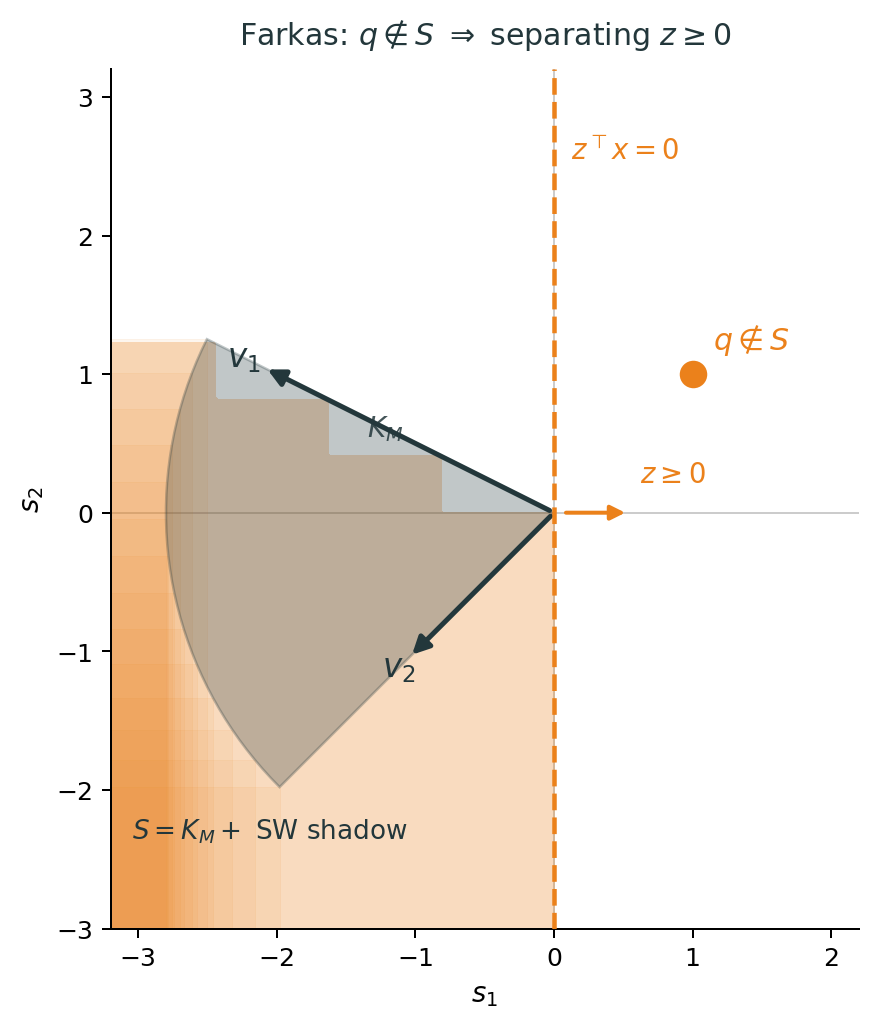
\includegraphics[width=0.72\textwidth]{figures/farkas_geometry.png}
\end{center}

\begin{proof}[Proof of Farkas' Lemma]
\emph{Step 1 (at most one alternative).}
Suppose both (i) and (ii) hold.
Pick $\mathbf{x}\ge\mathbf{0}$ with $M\mathbf{x}\ge\mathbf{q}$ and $\mathbf{z}\ge\mathbf{0}$ with
$M^{\mathsf T}\mathbf{z}\le\mathbf{0}$ and $\mathbf{q}^{\mathsf T}\mathbf{z}>0$.
Then
\[
  0 < \mathbf{q}^{\mathsf T}\mathbf{z}
  \le (M\mathbf{x})^{\mathsf T}\mathbf{z}
  = \mathbf{x}^{\mathsf T}(M^{\mathsf T}\mathbf{z})
  \le 0,
\]
a contradiction.

\emph{Step 2 (if (i) fails, then (ii) holds).}
If (i) fails, then $\mathbf{q}\notin S$.
Since $S$ is convex and closed, there exists $\mathbf{z}\neq\mathbf{0}$ with
$\mathbf{z}^{\mathsf T}\mathbf{s}\le 0$ for all $\mathbf{s}\in S$ and $\mathbf{z}^{\mathsf T}\mathbf{q}>0$.
For each standard basis vector $\mathbf{e}_i$, the point $-\mathbf{e}_i\in S$ (take $\mathbf{x}=\mathbf{0}$,
$\mathbf{y}=\mathbf{e}_i$), so $-z_i\le 0$, i.e.\ $z_i\ge 0$.
For each $\mathbf{x}\ge\mathbf{0}$, the point $M\mathbf{x}\in S$ (take $\mathbf{y}=\mathbf{0}$), so
$\mathbf{z}^{\mathsf T}M\mathbf{x}\le 0$, i.e.\ $M^{\mathsf T}\mathbf{z}\le\mathbf{0}$.
Thus (ii) holds.
\end{proof}

\econ{Either a target is feasible with free disposal, or a nonnegative price vector exposes it as
too ambitious---a no-arbitrage statement.}

With Farkas in hand, we can show that no strictly better dual bound is possible than the primal optimum.

\textbf{Strong duality.}

\begin{theorem}[Strong duality for LP]
If~\eqref{eq:primal} has an optimal value $p^*$, then~\eqref{eq:dual} has $d^*=p^*$.
\end{theorem}

\begin{proof}
Fix $\varepsilon>0$.
Because $p^*$ is optimal, no $\mathbf{x}\ge\mathbf{0}$ satisfies
$A\mathbf{x}\ge\mathbf{b}$ and $\mathbf{c}^{\mathsf T}\mathbf{x}\le p^*-\varepsilon$.
Equivalently, the system
\[
  A\mathbf{x}\ge\mathbf{b},\qquad
  \mathbf{c}^{\mathsf T}\mathbf{x}\le p^*-\varepsilon,\qquad
  \mathbf{x}\ge\mathbf{0}
\]
is infeasible.
Write this as $M\mathbf{x}\ge\mathbf{q}$ with
$M=\binom{A}{-\mathbf{c}^{\mathsf T}}$ and $\mathbf{q}=\binom{\mathbf{b}}{-(p^*-\varepsilon)}$.
By Farkas, (ii) holds: $\exists\,\mathbf{y}\ge\mathbf{0}$, $\mu\ge 0$ with
$A^{\mathsf T}\mathbf{y}-\mu\mathbf{c}\le\mathbf{0}$ and $\mathbf{b}^{\mathsf T}\mathbf{y}-\mu(p^*-\varepsilon)>0$.
If $\mu=0$, then $\mathbf{b}^{\mathsf T}\mathbf{y}>0$ while any primal feasible $\mathbf{x}$ gives
$\mathbf{b}^{\mathsf T}\mathbf{y}\le\mathbf{y}^{\mathsf T}A\mathbf{x}\le\mathbf{c}^{\mathsf T}\mathbf{x}$,
contradicting primal feasibility; hence $\mu>0$.
Divide by $\mu$ and set $\tilde{\mathbf{y}}=\mathbf{y}/\mu$.
Then $A^{\mathsf T}\tilde{\mathbf{y}}\le\mathbf{c}$ and $\mathbf{b}^{\mathsf T}\tilde{\mathbf{y}}>p^*-\varepsilon$,
so $\tilde{\mathbf{y}}$ is dual feasible with objective exceeding $p^*-\varepsilon$.
Since $\varepsilon>0$ was arbitrary, $d^*\ge p^*$.
Together with weak duality, $d^*=p^*$.
\end{proof}

\econ{\textbf{Minimum input cost = maximum output value} at optimality.
Efficient production can be supported by shadow output prices.}

Strong duality identifies the optimum value; complementary slackness identifies \emph{which} constraints matter at the optimum.

\textbf{Complementary slackness.}

\begin{theorem}[Complementary slackness]
Feasible $\mathbf{x},\mathbf{y}$ are optimal iff
\[
  (A\mathbf{x}-\mathbf{b})_i\,y_i = 0\ \forall i,
  \qquad
  (c-A^{\mathsf T}\mathbf{y})_j\,x_j = 0\ \forall j.
\]
\end{theorem}

In words:
\begin{center}
\small
\renewcommand{\arraystretch}{1.15}
\begin{tabular}{ll}
\toprule
\textbf{If \ldots} & \textbf{then \ldots} \\
\midrule
primal constraint $i$ is slack & $y_i=0$ \\
$y_i>0$ & primal constraint $i$ is tight \\
dual constraint $j$ is slack & $x_j=0$ \\
$x_j>0$ & dual constraint $j$ is tight \\
\bottomrule
\end{tabular}
\end{center}

\begin{proof}[Necessity]
Suppose $\mathbf{x},\mathbf{y}$ are optimal.
By strong duality, $\mathbf{c}^{\mathsf T}\mathbf{x}=\mathbf{b}^{\mathsf T}\mathbf{y}$.
In the weak-duality chain,
\[
  \mathbf{c}^{\mathsf T}\mathbf{x}
  \ge \mathbf{y}^{\mathsf T}A\mathbf{x}
  \ge \mathbf{b}^{\mathsf T}\mathbf{y},
\]
both inequalities must be equalities.
Hence $\mathbf{y}^{\mathsf T}(A\mathbf{x}-\mathbf{b})=0$ and $(\mathbf{c}-A^{\mathsf T}\mathbf{y})^{\mathsf T}\mathbf{x}=0$.
Each term in these dot products is a product of nonnegative factors, so every term must be zero.
\end{proof}

\begin{proof}[Sufficiency]
If complementary slackness holds, then
\[
  \mathbf{c}^{\mathsf T}\mathbf{x}
  = \mathbf{y}^{\mathsf T}A\mathbf{x} + (\mathbf{c}-A^{\mathsf T}\mathbf{y})^{\mathsf T}\mathbf{x}
  = \mathbf{y}^{\mathsf T}A\mathbf{x}
  = \mathbf{b}^{\mathsf T}\mathbf{y} + \mathbf{y}^{\mathsf T}(A\mathbf{x}-\mathbf{b})
  = \mathbf{b}^{\mathsf T}\mathbf{y}.
\]
Weak duality then certifies that both are optimal.
\end{proof}

\begin{remark}[Direct proof]
From $\mathbf{c}^{\mathsf T}\mathbf{x}=\mathbf{b}^{\mathsf T}\mathbf{y}$ and weak duality:
any feasible $\tilde{\mathbf{x}}$ has $\mathbf{c}^{\mathsf T}\tilde{\mathbf{x}}\ge\mathbf{c}^{\mathsf T}\mathbf{x}$;
any feasible $\tilde{\mathbf{y}}$ has $\mathbf{b}^{\mathsf T}\tilde{\mathbf{y}}\le\mathbf{b}^{\mathsf T}\mathbf{y}$.
\end{remark}

\econ{\textbf{Zero-profit / full-utilization} logic.
Output target slack $\Rightarrow$ zero shadow price; binding output target $\Rightarrow$ positive price.
Input not used $\Rightarrow$ $x_j=0$; input used $\Rightarrow$ breaks even at shadow output prices.
Links to the Day~3 producer-theory slide (efficient production supported by prices when free disposal holds).}

The derivation above used $\ge$ constraints and $\mathbf{x}\ge\mathbf{0}$.
The same bounding identity works for any mix of constraint and variable types; only the signs change.

\textbf{Dual of a general LP.}

\keyidea{Same bounding argument; signs follow from constraint and variable types.}

\begin{claim}[Dual rules for a general LP]
Consider a primal \textbf{minimisation} with any mix of $\ge$, $\le$, $=$ constraints and
nonnegative, nonpositive, or free variables.
The dual is a \textbf{maximisation} with one dual variable $y_i$ per primal constraint.
If the primal is a \textbf{maximisation}, reverse every inequality in the table below.
\end{claim}

\begin{proof}
For any primal feasible $\mathbf{x}$ and dual candidate $\mathbf{y}$,
\[
  \mathbf{c}^{\mathsf T}\mathbf{x}-\mathbf{b}^{\mathsf T}\mathbf{y}
  = (\mathbf{c}-A^{\mathsf T}\mathbf{y})^{\mathsf T}\mathbf{x}
    + \mathbf{y}^{\mathsf T}(A\mathbf{x}-\mathbf{b}).
\]
Require each bracketed term to be $\ge 0$ for \emph{all} primal feasible $\mathbf{x}$.
The sign of $y_i$ is pinned down by the type of primal constraint $i$;
the type of dual constraint on $(A^{\mathsf T}\mathbf{y})_j$ is pinned down by the sign of $x_j$.
Maximising $\mathbf{b}^{\mathsf T}\mathbf{y}$ subject to these conditions gives the dual.
The explicit rules for a primal minimum (dual maximum) are:
\begin{center}
\renewcommand{\arraystretch}{1.2}
\begin{tabular}{ll}
\toprule
\textbf{Primal} & \textbf{Dual} \\
\midrule
$\mathbf{a}_i^{\mathsf T}\mathbf{x}\ge b_i$ & $y_i\ge 0$ \\
$\mathbf{a}_i^{\mathsf T}\mathbf{x}\le b_i$ & $y_i\le 0$ \\
$\mathbf{a}_i^{\mathsf T}\mathbf{x}= b_i$ & $y_i$ free \\
$x_j\ge 0$ & $(A^{\mathsf T}\mathbf{y})_j\le c_j$ \\
$x_j\le 0$ & $(A^{\mathsf T}\mathbf{y})_j\ge c_j$ \\
$x_j$ free & $(A^{\mathsf T}\mathbf{y})_j= c_j$ \\
\bottomrule
\end{tabular}
\end{center}
\end{proof}

For example,
\[
  \min\ 3x_1-2x_2\ \text{ s.t. }\
  x_1+x_2\ge 5,\ 2x_1-x_2\le 10,\ x_1-3x_2=4,\ x_1\ge 0,\ x_2\ \text{free}
\]
has dual
\[
  \max\ 5y_1+10y_2+4y_3\ \text{ s.t. }\
  y_1+2y_2+y_3\le 3,\ y_1-y_2-3y_3=-2,\ y_1\ge 0,\ y_2\le 0,\ y_3\ \text{free}.
\]

Section~3 shows that this entire LP story is one instance of a broader Lagrangian construction.

%==============================================================================
\section{Lagrangian duality}
%==============================================================================

LP duality multiplies constraints by nonnegative weights, adds them to the objective, and maximises the
resulting lower bound.
The same recipe applies to nonlinear problems.
We proceed as follows: state the general primal and dual; prove weak duality; interpret the dual
geometrically in two settings; recover the LP dual from Section~2; and close with strong duality under
convexity and Slater's condition.

The general primal is
\[
  \text{(P)}\quad
  \min\ f_0(\mathbf{x})
  \ \text{s.t.}\ 
  f_i(\mathbf{x})\le 0,\ i=1,\ldots,m,\quad
  h_j(\mathbf{x})=0,\ j=1,\ldots,p,\quad
  \mathbf{x}\in D,
\]
with optimal value $p^*$.
The \textbf{Lagrangian} attaches multipliers to each constraint:
\[
  L(\mathbf{x},\boldsymbol{\lambda},\boldsymbol{\nu})
  = f_0(\mathbf{x})
  + \sum_{i=1}^m \lambda_i f_i(\mathbf{x})
  + \sum_{j=1}^p \nu_j h_j(\mathbf{x}),
  \qquad \boldsymbol{\lambda}\ge\mathbf{0},\ \boldsymbol{\nu}\ \text{free}.
\]
For any feasible $\mathbf{x}$, each added term is $\le 0$, so $L(\mathbf{x},\boldsymbol{\lambda},\boldsymbol{\nu})\le f_0(\mathbf{x})$.
The \textbf{dual function} minimises the Lagrangian over $\mathbf{x}$:
\[
  g(\boldsymbol{\lambda},\boldsymbol{\nu})
  = \inf_{\mathbf{x}\in D} L(\mathbf{x},\boldsymbol{\lambda},\boldsymbol{\nu}).
\]
The \textbf{dual problem} chooses multipliers to sharpen this bound:
\[
  \text{(D)}\quad \max\ g(\boldsymbol{\lambda},\boldsymbol{\nu})\ \text{s.t.}\ \boldsymbol{\lambda}\ge\mathbf{0},
  \qquad d^* = \sup_{\boldsymbol{\lambda}\ge\mathbf{0}} g(\boldsymbol{\lambda},\boldsymbol{\nu}).
\]

\begin{theorem}[Weak duality for the Lagrangian dual]
Always $g(\boldsymbol{\lambda},\boldsymbol{\nu})\le p^*$ for $\boldsymbol{\lambda}\ge\mathbf{0}$, hence $d^*\le p^*$.
The quantity $p^*-d^*$ is the \textbf{duality gap}.
\end{theorem}

\begin{proof}
For any primal feasible $\mathbf{x}$ and any $\boldsymbol{\lambda}\ge\mathbf{0}$, $\boldsymbol{\nu}$,
\[
  g(\boldsymbol{\lambda},\boldsymbol{\nu})
  \le L(\mathbf{x},\boldsymbol{\lambda},\boldsymbol{\nu})
  = f_0(\mathbf{x}) + \sum_i \lambda_i f_i(\mathbf{x}) + \sum_j \nu_j h_j(\mathbf{x})
  \le f_0(\mathbf{x}),
\]
because $f_i(\mathbf{x})\le 0$, $h_j(\mathbf{x})=0$, and $\lambda_i\ge 0$.
Taking the infimum over primal feasible $\mathbf{x}$ on the right gives
$g(\boldsymbol{\lambda},\boldsymbol{\nu})\le p^*$.
Maximising over $\boldsymbol{\lambda},\boldsymbol{\nu}$ yields $d^*\le p^*$.
\end{proof}

Pictures make the dual function easy to remember: it is the intercept of the best supporting line or
hyperplane below the cloud of all achievable constraint--objective pairs.

\textbf{Geometry I: one inequality and the \texorpdfstring{$(u,t)$}{(u,t)} cloud.}
\keyidea{Dual $=$ best lower bound from a supporting \textbf{line} below the whole achievable set
$\mathcal{A}\subset\mathbb{R}^2$.}

Consider $\min_{\mathbf{x}}\ f_0(\mathbf{x})$ s.t.\ $f_1(\mathbf{x})\le 0$.
Write $u=f_1(\mathbf{x})$ and $t=f_0(\mathbf{x})$.
As $\mathbf{x}$ runs over $D$, the pairs
\[
  \mathcal{A}=\{\,(u,t):\ u=f_1(\mathbf{x}),\ t=f_0(\mathbf{x}),\ \mathbf{x}\in D\,\}
\]
form the \textbf{whole cloud} of achievable outcomes, both feasible ($u\le 0$) and infeasible.
The primal value $p^*$ is the smallest $t$ among points in $\mathcal{A}$ with $u\le 0$.
For $\lambda\ge 0$, lines $t+\lambda u=\alpha$ have slope $-\lambda$ in the $(u,t)$ plane, and
\[
  g(\lambda)=\inf_{(u,t)\in\mathcal{A}}(t+\lambda u)
\]
is the smallest $\alpha$ such that the line still touches $\mathcal{A}$ from below (its intercept on $u=0$).
The infimum is over \textbf{all} of $\mathcal{A}$, not only the feasible slice $u\le 0$.

\begin{claim}[Geometric weak duality in the \texorpdfstring{$(u,t)$}{(u,t)} picture]
For every $\lambda\ge 0$, $g(\lambda)\le p^*$.
The dual value $d^*=\sup_{\lambda\ge 0} g(\lambda)$ is the largest intercept at $u=0$ obtained by a
supporting line below $\mathcal{A}$.
\end{claim}

\begin{proof}
Take any feasible point $(u,t)\in\mathcal{A}$ with $u\le 0$.
Since $\lambda\ge 0$, $t+\lambda u\le t$.
Also $g(\lambda)\le t+\lambda u$ by definition of the infimum.
Hence $g(\lambda)\le t$.
Minimising $t$ over feasible points gives $g(\lambda)\le p^*$.
Maximising $g(\lambda)$ over $\lambda\ge 0$ gives $d^*$.
\end{proof}

\begin{center}
  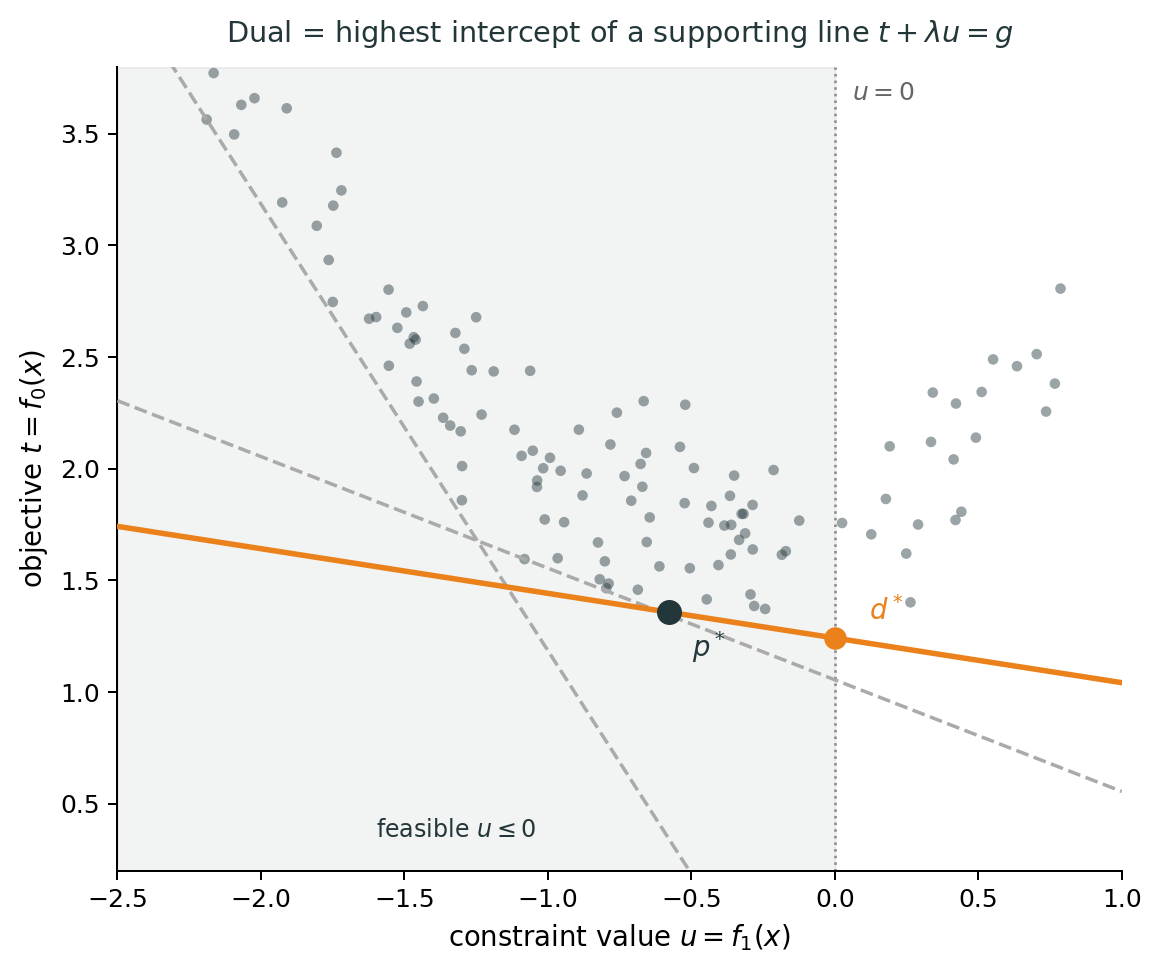
\includegraphics[width=0.78\textwidth]{figures/lagrange_geometry.png}
\end{center}

\textbf{Geometry II: one inequality, one equality, and the \texorpdfstring{$(u,v,t)$}{(u,v,t)} cloud.}
\keyidea{Adding an equality lets the supporting object tilt in a \textbf{third} direction; free $\nu$ can
tighten the bound.}

Now add $h(\mathbf{x})=0$ and write $u=f_1(\mathbf{x})$, $v=h(\mathbf{x})$, $t=f_0(\mathbf{x})$.
The cloud
\[
  \mathcal{A}=\{\,(u,v,t):\ u=f_1(\mathbf{x}),\ v=h(\mathbf{x}),\ t=f_0(\mathbf{x}),\ \mathbf{x}\in D\,\}
\]
again contains \textbf{all} achievable triples; feasible points satisfy $u\le 0$ and $v=0$.
Among them, the primal minimises $t$, giving $p^*$.
Choose $\lambda\ge 0$ (for $u$) and $\nu$ free (for $v$). The plane $t+\lambda u+\nu v=\alpha$ supports $\mathcal{A}$ from below, and
\[
  g(\lambda,\nu)=\inf_{(u,v,t)\in\mathcal{A}}(t+\lambda u+\nu v)
\]
is its intercept at $u=0$, $v=0$.

\begin{claim}[Geometric weak duality in the \texorpdfstring{$(u,v,t)$}{(u,v,t)} picture]
For every $\lambda\ge 0$ and $\nu$, $g(\lambda,\nu)\le p^*$.
The dual problem $d^*=\sup_{\lambda\ge 0,\,\nu} g(\lambda,\nu)$ seeks the best intercept from a hyperplane below the full cloud $\mathcal{A}$.
\end{claim}

\begin{proof}
For any feasible $(u,v,t)$, $u\le 0$ and $v=0$, so $t+\lambda u+\nu v=t+\lambda u\le t$.
Since $g(\lambda,\nu)\le t+\lambda u+\nu v$, we get $g(\lambda,\nu)\le p^*$.
\end{proof}

\begin{remark}[Why $\nu=0$ can be weaker]
With $\nu=0$, the plane $t+\lambda u=\alpha$ cannot tilt in the $v$-direction.
The infimum $g(\lambda,0)$ may occur at $v\neq 0$, giving a low intercept at $v=0$.
Allowing $\nu$ to vary lets the plane tilt so the minimum over $\mathcal{A}$ can occur nearer $v=0$,
often raising the bound; for convex problems this can achieve $d^*=p^*$.
For LPs, $\mathcal{A}$ is a polyhedron (convex), so strong duality holds when the primal optimum is finite.
\end{remark}

Having seen the geometry, we verify that the LP dual of Section~2 is exactly what the Lagrangian recipe produces.

\textbf{LP recovers Section~2.}

\begin{claim}[LP Lagrangian dual equals the LP dual]
Write $\min\ \mathbf{c}^{\mathsf T}\mathbf{x}$ s.t.\ $A\mathbf{x}\ge\mathbf{b}$, $\mathbf{x}\ge\mathbf{0}$ as
$f_0(\mathbf{x})=\mathbf{c}^{\mathsf T}\mathbf{x}$,
$f_1(\mathbf{x})=\mathbf{b}-A\mathbf{x}\le\mathbf{0}$,
$f_2(\mathbf{x})=-\mathbf{x}\le\mathbf{0}$.
The Lagrangian dual~\eqref{eq:dual} is obtained with $\mathbf{y}=\boldsymbol{\lambda}$.
\end{claim}

\begin{proof}
The Lagrangian is
\[
  L=\mathbf{c}^{\mathsf T}\mathbf{x}+\boldsymbol{\lambda}^{\mathsf T}(\mathbf{b}-A\mathbf{x})
  +\boldsymbol{\mu}^{\mathsf T}(-\mathbf{x}).
\]
For fixed $(\boldsymbol{\lambda},\boldsymbol{\mu})$,
\[
  g(\boldsymbol{\lambda},\boldsymbol{\mu})
  = \inf_{\mathbf{x}}\bigl[(\mathbf{c}-A^{\mathsf T}\boldsymbol{\lambda}-\boldsymbol{\mu})^{\mathsf T}\mathbf{x}
  +\boldsymbol{\lambda}^{\mathsf T}\mathbf{b}\bigr].
\]
If $A^{\mathsf T}\boldsymbol{\lambda}+\boldsymbol{\mu}\neq\mathbf{c}$, the infimum is $-\infty$.
If $A^{\mathsf T}\boldsymbol{\lambda}+\boldsymbol{\mu}=\mathbf{c}$, then $g=\boldsymbol{\lambda}^{\mathsf T}\mathbf{b}$.
Requiring $\boldsymbol{\lambda}\ge\mathbf{0}$ and $\boldsymbol{\mu}\ge\mathbf{0}$ and writing
$A^{\mathsf T}\boldsymbol{\lambda}\le\mathbf{c}$ gives~\eqref{eq:dual} with $\mathbf{y}=\boldsymbol{\lambda}$.
\end{proof}

When the problem is convex and strictly feasible, weak duality upgrades to strong duality.

\textbf{Strong duality for convex problems.}
The problem is \textbf{convex} if $f_0,f_i$ are convex, $h_j$ are affine, and $D$ is convex.

\begin{theorem}[Strong duality]
If the primal is convex, \textbf{Slater's condition} holds (strict feasibility:
$f_i(\mathbf{x})<0$, $h_j(\mathbf{x})=0$ for some $\mathbf{x}\in\mathrm{relint}\,D$),
and $p^*$ is finite, then $d^*=p^*$ and the dual optimum is attained.
\end{theorem}

\begin{remark}[What is $\mathrm{relint}\,D$?]
The \textbf{relative interior} $\mathrm{relint}\,D$ is the ``interior'' of $D$ measured inside the
flat (affine hull) that contains $D$, not inside all of $\mathbb{R}^n$.
\begin{itemize}[nosep,leftmargin=*]
  \item If $D=\mathbb{R}^n$, then $\mathrm{relint}\,D=\mathbb{R}^n$.
  \item If $D$ is a line segment in $\mathbb{R}^2$, its usual topological interior is empty,
        but $\mathrm{relint}\,D$ is the \textbf{open segment} (endpoints excluded).
  \item If $D=\{\mathbf{x}:A\mathbf{x}\le\mathbf{b}\}$ is a full-dimensional polyhedron,
        $\mathrm{relint}\,D$ is the set of points that satisfy every inequality \textbf{strictly}
        ($A\mathbf{x}<\mathbf{b}$), i.e.\ not on a lower-dimensional face.
\end{itemize}
Slater asks for a \textbf{strictly feasible} point that is not trapped on a boundary of $D$:
inequalities hold with slack ($f_i(\mathbf{x})<0$), equalities hold exactly, and $\mathbf{x}$ lies
in the relative interior of the domain.
\end{remark}

For LPs, a feasible point with finite optimum suffices.
Slater is the convex analogue of ``interior point exists.''

\econ{$\lambda_i,\nu_j$ are shadow prices on constraints.
The dual finds the price system giving the best accounting lower bound on optimal cost.
When the gap vanishes, prices fully explain the optimum.}

\end{document}
